\documentclass{article}
\usepackage{college-math-j}
\usepackage{xfrac}
\usepackage{textcomp}


%MAKING THE CAVALIERI INTEGRAL NOTATION
%%%%%%%%%%%%%%%%%%%%%%%%%%%%%%%%%%%%%%%
\makeatletter
%\let\DOTSI\relax % amsmath support for \dots
\newcommand*{\cint}{%
  \DOTSI
  \mathop{%
    \mathpalette\@LetterOnInt{\mathbf{c}}%
  }%
  \mkern-\thinmuskip % thin space is inserted between two \mathop
  \int
}
\newcommand*{\@LetterOnInt}[2]{%
  \sbox0{$#1\int\m@th$}%
  \sbox2{$%
    \ifx#1\displaystyle
      \textstyle
    \else
      \scriptscriptstyle
    \fi
    #2%
  \m@th$}%
  \dimen@=.4\dimexpr\ht0+\dp0\relax
  \ifdim\dimexpr\ht2+\dp2\relax>\dimen@
    \sbox2{\resizebox*{!}{\dimen@}{\unhcopy2}}%
  \fi
  \dimen@=\wd0 %
  \ifdim\wd2>\dimen@
    \dimen@=\wd2 %
  \fi
  \rlap{\hbox to \dimen@{\hfil
    $#1\vcenter{\copy2}\m@th$%
  \hfil}}%
  \ifdim\dimen@>\wd0 %
    \kern.5\dimexpr\dimen@-\wd0\relax
  \fi
}
\makeatother
%%%%%%%%%%%%%%%%%%%%%%%%%%%%%%%%%%%%%%%


%% IF YOU HAVE FONTS INSTALLED
%\usepackage{mtpro}
%\usepackage{mathtime}

\theoremstyle{theorem}
\newtheorem{theorem}{Theorem}

\theoremstyle{definition}
\newtheorem*{definition}{Definition}
\newtheorem*{remark}{Remark}

\begin{document}

\title{Computing volume via non-linear rectangular infinitesimals}
%\author{Woodrow Wilson and Herbert Hoover} %%leave blank in initial submission to allow for double blind reviewing
%\author{ }

\maketitle

%Notes authors should leave bios out altogether.

%\begin{biog} %comment out in initial submission to allow for double blind reviewing
%\item[\biogpic{\includegraphics[width=84pt]{Woodrow_Wilson.pdf}}Woodrow Wilson] (twwilson@princeton.edu) received his PhD in history and political science from Johns Hopkins University. He held visiting positions at Cornell and Wesleyan before joining the faculty at Princeton, where he was eventually appointed president of the university.  Among his proudest accomplishments was the abolition of eating clubs at Princeton on the grounds that they were elitist.

%\item[\biogpic{\includegraphics[width=84pt]{Herbert_Hoover.pdf}}Herbert Hoover] (hchoover@stanford.edu) entered Stanford University in 1891, after failing all of the entrance exams except mathematics.  He received his BS degree in geology in 1895, spent time as a mining engineer, then was appointed by his co-author to the U.S. Food Administration and the Supreme Economic Council, where he orchestrated the greatest famine relief efforts of all time.
%\end{biog}
%This is not to say that there  This is partly, because there is no simplistic geometric interpretation for fractional calculus.  
\noindent
Bonaventura Cavalieri was a mathematician who lived in the 17th century. He made numerous contributions to the fields of optics, astronomy and geometry. 
Cavalieri was a student of Galileo. He served as a professor of mathematics at the university of Bologna from 1629 until his death in 1647. 
Galileo held Cavalieri in high esteem as is evedent from the following extract of a reference letter Galileo wrote in which he recommended Cavalieri for the chair of mathematics at Bologna: ``\emph{few, perhaps none, from 
Archimedes onwards, have investigated so deeply and have entered so far into the science of geometry}''. In 1935, a moon crater, Cavalerius, was officially named after him to commemorate his achievements and to honor his memory (see Fig ) \cite{?}. 
\begin{figure}[htb]
\centering
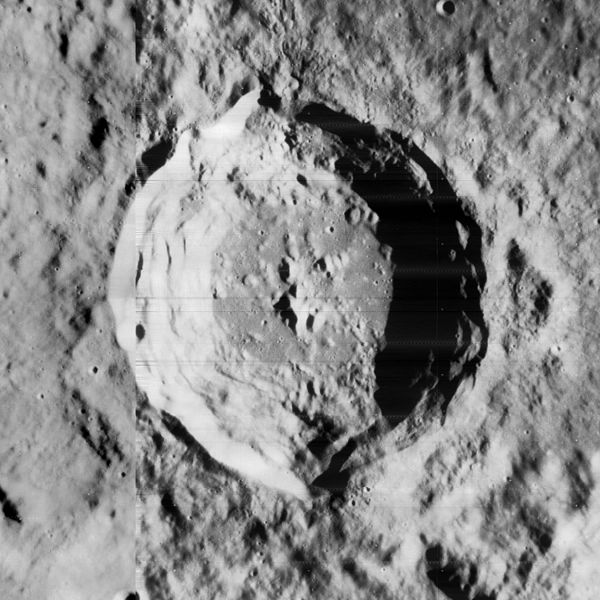
\includegraphics[width=0.4\textwidth]{crater.jpg}
\caption{xx}
\label{fig:crater}
\end{figure}
Cavalieri's most notable achievement was the publication of his 
treatise, \emph{Geometria indivisibilibus}, in which he describes the precalculus method of indivisibles. The method of indivisibles can be attributed to the ancient Greeks,
in this case Democritus and Archimedes. The method is used to compute the area and the volume of complex planar figures and solids, respectively.
It works by finding a planar figure or a solid, whose area or volume can easily be computed, which is Cavalieri congruent to a planar figure or solid whose 
area or volume is unknown. Two planar figures or solids are Cavalieri congruent if they can be decomposed into the same set of parallel ``indivisibles''. An indivisible of 
a planar figure is any cord of the planar figure. An indivisible of a solid is any planar section of a solid. Two indivisibles are equal if they are of the same length or area.
It is Cavalieri's principle that assures us that two planar figures or solids that are composed of the same set of indivisibles have equal area or volume. Cavalieri's principle 
in $\mathbb{R}^3$ is stated below without proof:

\begin{theorem}[Cavalieri's principle in $\mathbb{R}^3$]
If two solids are included between a pair of parallel planes, and if the areas of
the two sections cut by them on any plane parallel to the including planes are always
equal, then the volumes of the two solids are equal.
\end{theorem}

\begin{figure}[htb]
\centering
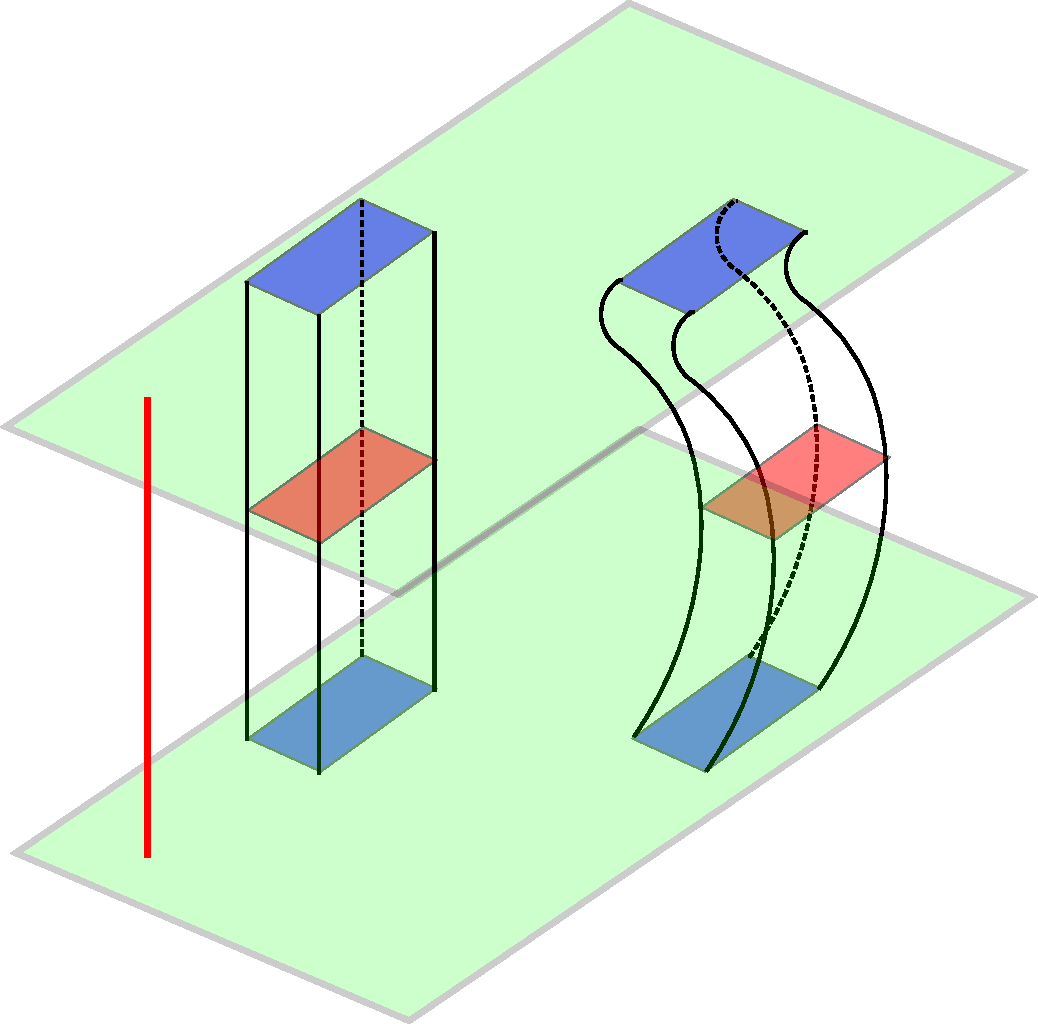
\includegraphics[width=0.5\textwidth]{cav_principle.pdf}
\caption{xx}
\label{fig:cav_principle}
\end{figure}



\noindent
Fig~\ref{??} depicts a classic rectangular prism or column as well as a \emph{non-linear rectangular prism or column}. The volumes of the two solids in Fig~\ref{??} are equal due 
to Cavalieri's principle. Note that in this article we use the non-standerdized term non-linear rectangular prism or column to refer to a solid that has a rectangular 
base and lateral edges that are non-linear and translations of one another.

\section{Cavalieri Integral}
The single Cavalieri integral was originally defined in \cite{ackermann12} without having to resort to vector calculus. In this section we will redefine the Cavalieri integral using vector calculus notation. As the reader will undoubtedly realize, if we define the single Cavalieri integral using vector calculus then it becomes trivial to
extend its definition into $\mathbb{R}^3$.\\

%In this section we define the Cavalieri integral \cite{ackermann12}. 

\noindent
Consider the curve $f(x)$, the curve $\mathbf{c}(t)=\left <c_x(t),c_y(t) \right >$ and the interval $[a,b]$.

\begin{definition}[Translational curve in $\mathbb{R}^2$]
If a curve $\mathbf{c}(t)$ in $\mathbb{R}^2$ intersects the $x$ axis at the origin and $\mathbf{c}(t) + \left < e,0 \right >$ intersects 
the curve $f(x)$ at a single point for all $e\in [a,b]$ then $\mathbf{c}(t)$ is a translational curve 
with respect to $f(x)$ on $[a,b]$. 
\end{definition}

\noindent
Moreover, assume that $\mathbf{c}(t)$ is a translational curve with respect to $f(x)$ on $[a,b]$. Let us first partition $[a,b]$ into $n$ subintervals $[x_{i},x_{i+1}]$ of equal 
width $\Delta x^1 = \Delta x_i^1 = x_{i+1}-x_i\ll (b-a)$. Furthermore, let the transformation function $h$ map the $x$--coordinate $x_i^1\in [a,b]$ at which $\mathbf{c}(t) + \left <x_i^1,0 \right >$ intersects the 
$x$-axis to the $x$--coordinate at which $\mathbf{c}(t) + \left <x_i^1,0 \right >$ intersects $f(x,y)$. Note, the domain of $h$ is $[a,b]$. Let $a'$ denote the $x$-coordinate 
at which $\mathbf{c}(t) + \left <a,0 \right >$ intersects $f(x,y)$ and let $b'$ denote the $x$-coordinate 
at which $\mathbf{c}(t) + \left <b,0 \right >$ intersects $f(x,y)$.  Note, the range 
of $h$ is $[a',b']$. As the partition of $[a,b]$ can be made arbitrarily fine, $h:[a,b]\rightarrow [a',b']$ actually maps every point $x_i^1\in [a,b]$ to a point $x_i^2\in [a',b']$. \\

\noindent
Let $R$ denote the region which is bounded by $f(x,y)$, $\mathbf{c}(t)+\left <a,0\right >$, $\mathbf{c}(t)+\left <b,0\right >$ and the $x$-axis. 
As an example, the region $R$ depicted in Figure~\ref{fig:caval2} is obtained if we set $f(x) = x$, $\mathbf{c}(t) = \left<-\frac{1}{2} t,\frac{1}{2} t\right>$, $a = 1$ and $b = 4$.
Let $A_R$ denote the area of $R$. We can approximate $A_R$ with:
\begin{equation}
 \label{eq:caval1}
 A_R \approx \sum_{i=0}^{n-1} f(x_i^2)\Delta x_i^1,
 \end{equation}
Let us verify that this is indeed the case. If we closely inspect Equation~\ref{eq:caval1} and Figure~\ref{fig:caval2} we notice the following:
 \begin{itemize}
  \item $\Delta x_i^1 = x_{i+1}^1 - x_i^1$ represents the width of a non-rectangular integration strip.
  \item $f(x_i^2)$ represents the height of a non-rectangular integration strip.
  \item $f(x_i^2)\Delta x_i^1$ represents the area of a non-rectangular integration strip (due to Cavalieri's principle).
  \item The Cavalieri sum $\sum_{i=0}^{n-1} f(x_i^2)\Delta x_i^1$, therefore, approximates the area of $R$.
  \item In the limit the Cavalieri sum (if this limit exists), therefore, approaches the area of $R$.
 \end{itemize}

\begin{figure}[htb]
\centering
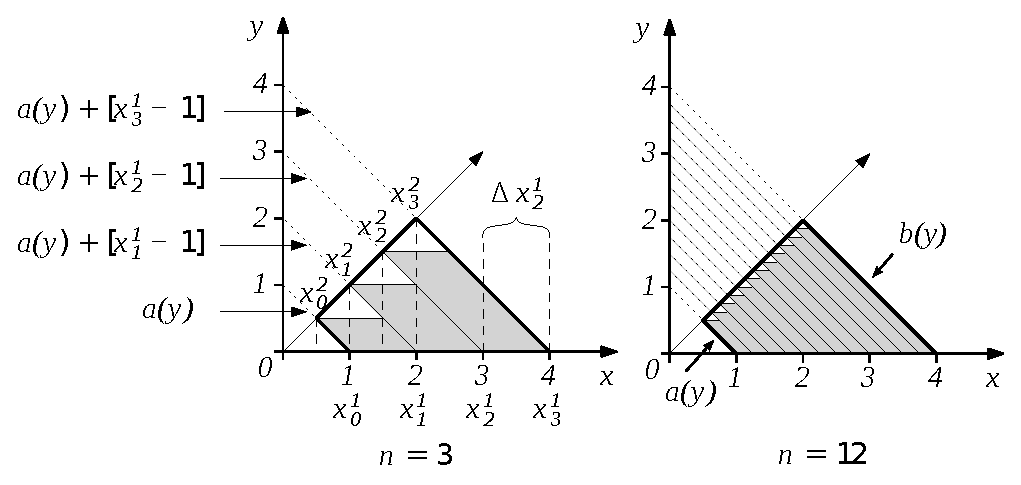
\includegraphics[width=0.75\textwidth]{fig13.eps}
\caption{Region bounded by the $x$-axis and the lines $f(x)=x$, $a(y)=1-y$, and $b(y)=4-y$. The figure also depicts the partition points $x_i^1$ and $x_i^2$ as used in the Cavalieri sum (see Eq.~\eqref{eq:cav_sum}). Reproduced from Quaestiones Mathematicae (2012) 35: 265-296 with permission \copyright~ NISC (Pty) Ltd.}
\label{fig:caval2}
\end{figure}

\noindent
The aforementioned limit is known as the Cavalieri integral and in this paper we denote this integral as follows:

\begin{equation}
\label{eq:cav_1d}
\int \limits_{\mathcal{C}} f(x)~dx = \lim_{n \rightarrow \infty}  \sum_{i=0}^{n-1} f(x_i^2) \Delta x_i^1,
\end{equation}
with $\mathcal{C} = \{\mathbf{c}(t),[a,b]\}$. Equation~\eqref{eq:cav_1d} is difficult to evaluate in its current form. Luckily, the Cavalieri integral 
can be converted into an equivalent Riemann integral using the transformation $h$:
 \begin{equation}
 \int \limits_{\mathcal{C}} f(x)\, dx = \int_{a}^{b} f\circ h(x)~dx. 
\end{equation}

\noindent
The only thing that now remains is to find an expression for $h$. Note that, for every coordinate $(x_i^1,x_i^2) \in [a,b] \times [a',b']$ there exists a unique $t\in\mathbb{R}$ such that
\begin{equation}
 \label{eq:pat_rel_1d}
 \left <x_i^2,f(x_i^2) \right > = \left <x_i^1,0 \right> + \left<c_x(t),c_y(t) \right >.
 \end{equation}
 We can rewrite Equation~\eqref{eq:pat_rel_1d} as
 \begin{equation}
 \label{eq:t_func_1d}
 c_y(t) = f(x_i^1 + c_x(t)).
 \end{equation}
 We can now solve for $t$ in Equation~\eqref{eq:t_func_1d} in terms of $x_i^1$. If we substitute the solution $t(x_i)$ so obtained into Equation~\ref{eq:pat_rel_1d} we obtain 
\begin{equation}
\label{eq:h_func_1d}
 x_i^2 = h(x_i^1) = x_i^1 + c_x\circ t(x_i^1).
\end{equation}

\noindent
Note, the Cavalieri integral is denoted in \cite{ackermann12} via:
\begin{equation}
\label{eq:cav_1d}
\int_{a(y)}^{b(y)} f(x)~dx = \lim_{n \rightarrow \infty}  \sum_{i=0}^{n-1} f(x_i^2) \Delta x_i^1,
\end{equation}
where $a(y)$ denotes the functional representation of $\mathbf{c}(t) + \left <a,0 \right >$ and $b(y) = a(y)+(b-a)$.






%Let the region $R$ be bounded by the $x$-axis and the lines $f(x)=x$, $a(y)=1-y$ and $b(y)=4-y$. This region is shown in Fig.~\ref{fig:caval2}.\\
%\begin{figure}[htb]
%\centering
%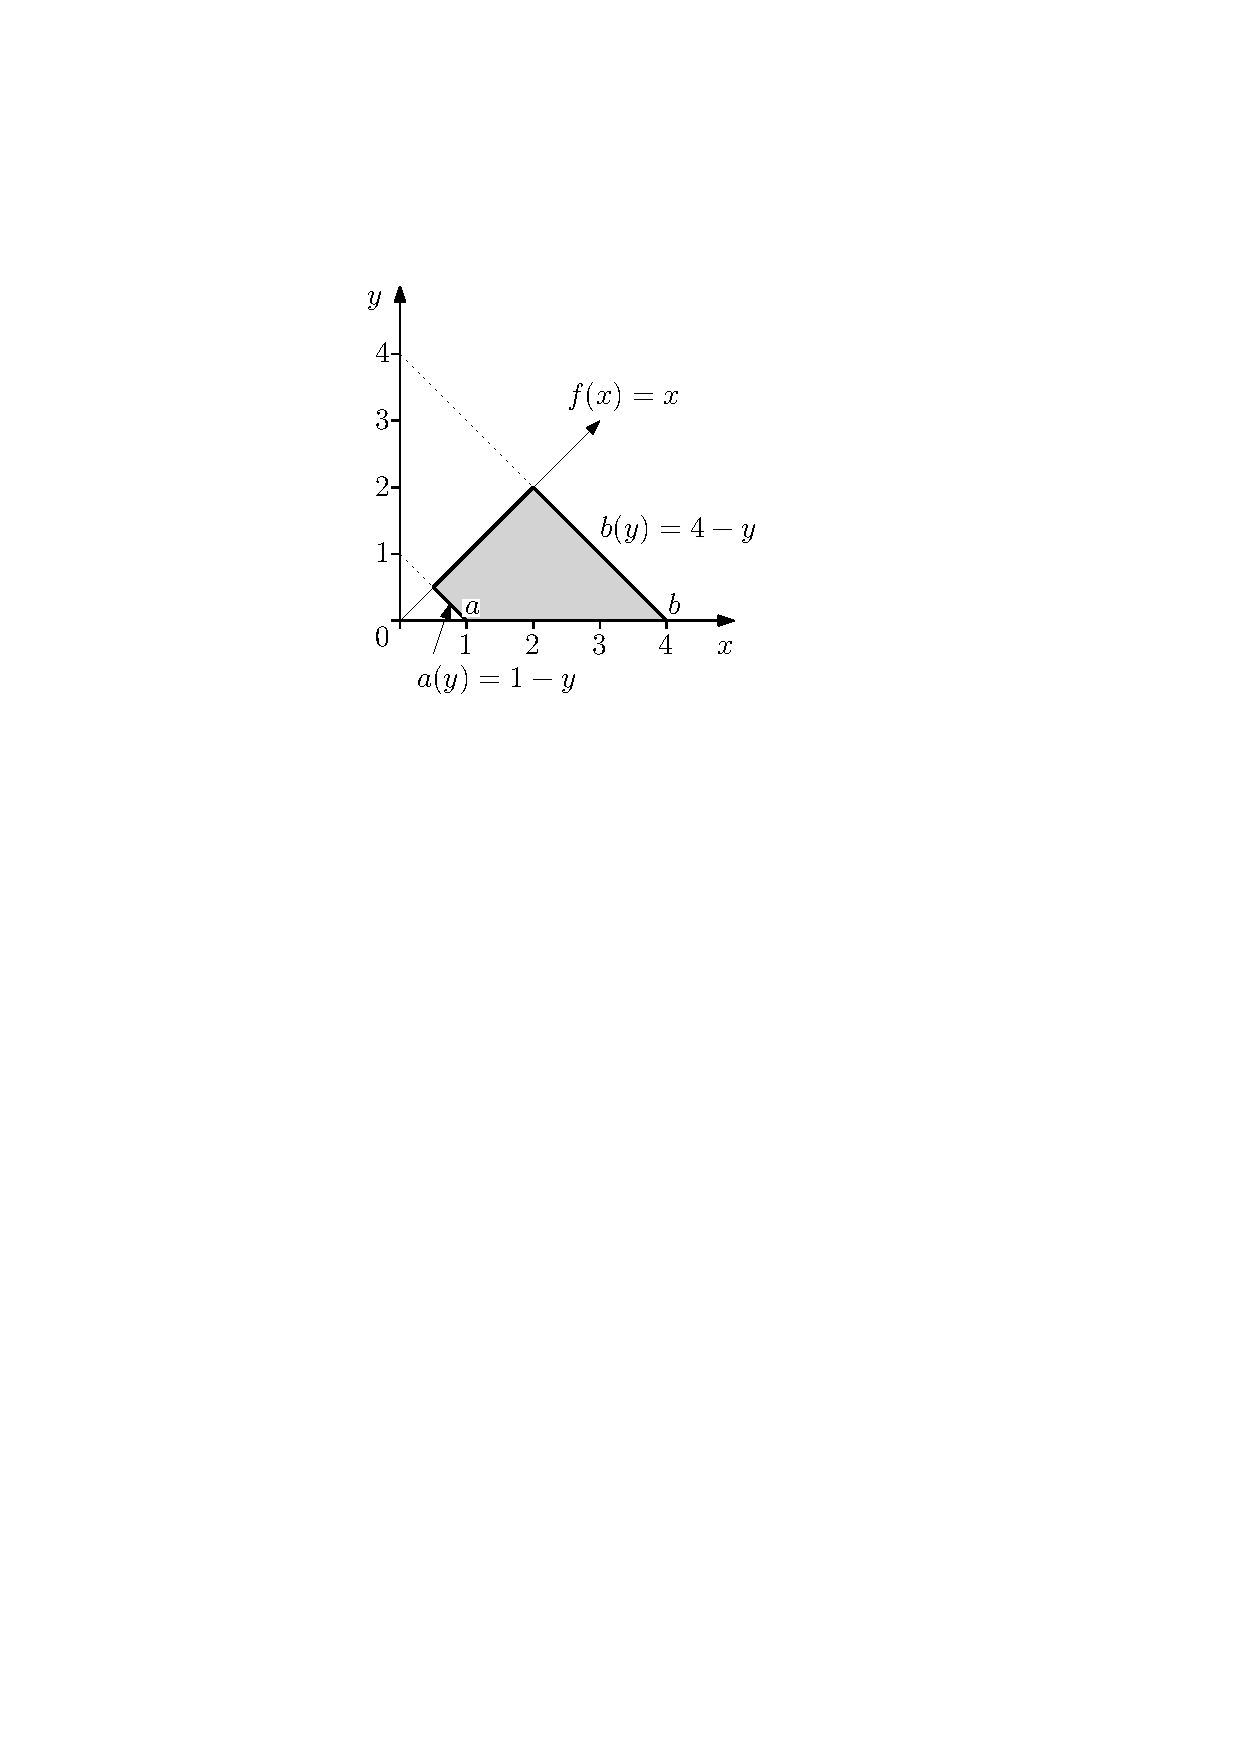
\includegraphics[width=0.3\textwidth]{fig12}
%\caption{Region bounded by the $x$-axis and the lines $f(x)=x$, $a(y)=1-y$, and $b(y)=4-y$. Reproduced from Quaestiones Mathematicae (2012) 35: 265-296 with permission \copyright~ NISC (Pty) Ltd.}
%\label{fig:ex1}
%\end{figure}

% \noindent
% We can compute the area of $R$ as follows:
% \begin{equation}
% \int_0^2x\, dx+\int_2^44-x\, dx- \int_0^{\frac{1}{2}}x\, dx-\int_{\frac{1}{2}}^11-x\, dx = 3.75. 
% \end{equation}
% 
% \noindent
% Alternatively, the area of $R$ can also be determined via the Cavalieri integral:
% \begin{equation}
% \label{eq:caval1}
% \int_{a(y)}^{b(y)}f(x)\, dx = \lim_{n\to \infty}\sum_{i=0}^{n-1} f(x_i^2)\Delta x_i^1,
% \end{equation}
% with $\Delta x_i^1 = x_{i+1}^1 - x_i^1$. Furthermore, the partition points $(x_i^1)_{i=0}^{n}$ and $(x_i^2)_{i=0}^{n}$ are depicted in Fig.~\ref{fig:caval2}. Let us review why this is in fact the case:
% \begin{itemize}
%  \item $\Delta x_i^1 = x_{i+1}^1 - x_i^1$ represents the width of a non-rectangular integration strip.
%  \item $f(x_i^2)$ represents the height of a non-rectangular integration strip.
%  \item $f(x_i^2)\Delta x_i^1$ represents the area of a non-rectangular integration strip (due to Cavalieri's principle).
%  \item The Cavalieri sum $\sum_{i=0}^{n-1} f(x_i^2)\Delta x_i^1$, therefore, approximates the area of $R$.
%  \item In the limit the Cavalieri sum, therefore, approaches the area of $R$.
% \end{itemize}
% 
% \noindent
% The Cavalieri integral is, however, hard to evaluate directly. Fortunately, it is easy to convert a Cavalieri integral into an equivalent Riemann integral:
% \begin{equation}
% \int_{a(y)}^{b(y)}f(x)\, dx = \int_{a}^{b} f\circ h(x)~dx, 
% \end{equation}
% with $a(0) = a$ and $b(0)=b$. The function $h$ is known as the transformation function and it maps $x_i^1\in[a,b]$ to $x_i^2\in[a',b']$. It can be constructed via the function $g(x) = x - a\circ f(x) + a$ as 
% $h=g^{-1}$.
% 
% \noindent
% The area of $R$ can, therefore, also be computed as follows:
% \begin{equation}
% \int_{a(y)}^{b(y)}f(x)\, dx = \int_a^b f \circ h (x)\, dx = \dfrac{1}{2}\int_1^4x\, dx = 3.75.  
% \end{equation}
% 
% Let $\mathbf{c}(t) = \left <c_x(t),c_y(t) \right>$ be the vector equation of $a(y)-a$. The notation which we have been using to denote a Cavalieri integral up until now 
% in the paper was first proposed by Ackermann. Going forward in this paper, however, we propose making use of the following alternative notation:
% \begin{equation}
% \label{eq:new_def_cavalieri}
% \int \limits_{\mathcal{C}} f(x)~dx := \int_{a(y)}^{b(y)}f(x)~dx,
% \end{equation}
% with $\mathcal{C} = \{\mathbf{c}(t),[a,b]\}$. Note that $\left<a,0\right> + \mathbf{c}(t)$ and $\left<b,0\right> + \mathbf{c}(t)$ are the vector equations of $a(y)$ and 
% $b(y)$. The reason for this change in notation will become clear to the reader at a later stage. In turns out, that we can use $\mathbf{c}(t)$ to construct $h(x)$ via:
% \begin{equation}
% \label{eq:h_func}
% x_i^2 = h(x_i^1) = x_i^1 + c_x\circ t(x_i^1).
% \end{equation}
% 
% \noindent
% We will now show that this is indeed the case. Note that, for every coordinate $(x_i^1,x_i^2) \in [a,b] \times [a',b']$ there exists a unique $t\in\mathbb{R}$ such that
% \begin{equation}
% \label{eq:pat_rel}
% \left <x_i^2,f(x_i^2) \right > = \left <x_i^1,0 \right> + \left<c_x(t),c_y(t) \right >.
% \end{equation}
% We can rewrite Equation~\eqref{eq:pat_rel} as
% \begin{equation}
% \label{eq:t_func}
% c_y(t) = f(x_i^1 + c_x(t)).
% \end{equation}
% We can now solve for $t$ in Equation~\eqref{eq:t_func} in terms of $x_i^1$. If we substitute the solution $t(x_i)$ so obtained into Equation~\ref{eq:pat_rel} we obtain Equation~\ref{eq:h_func}.
% 
% In the case of $R$ we have that $\mathbf{c}(t) = \left<-\frac{1}{2} t,\frac{1}{2} t\right>$. If we solve for $t$ in terms of $x_i^1$ after having substituted $\mathbf{c}(t)$ into Eq we obtain 
% $t(x_i^1) = x_i^1$. If we now substitute our solution $t(x_i^1)$ into Eq we obtain, as required, $h(x_i^1) = \frac{1}{2}x_i^2$. This result, therefore, validates Eq ??.

\section{Double Cavalieri Integral}
In this section we define the double Cavalieri integral and we show that it can be used to calculate the volume of solids that can be decomposed into an infinite 
number of non-linear regtangular infinitesimals.\\

\noindent
Without the loss of generality, consider the surface $f(x,y)$, the curve $\mathbf{c}(t)$\\$=\left <c_x(t),c_y(t), c_z(t) \right >$ and the region $R = [a,b]\times [c,d] = \{(x,y)\in \mathbb{R}^2|a \leq x \leq b, c \leq y \leq d\}$.

\begin{definition}[Translational curve in $\mathbb{R}^3$]
If a curve $\mathbf{c}(t)$ in $\mathbb{R}^3$ intersects the $xy$ plane at the origin and $\mathbf{c}(t) + \left < e,f,0 \right >$ intersects 
the surface $f(x,y)$ at a single point for all $(e,f)\in R$ then $\mathbf{c}(t)$ is a translational curve 
with respect to $f(x,y)$ on $R$. 
\end{definition}

\noindent
Moreover, assume that $\mathbf{c}(t)$ is a translational curve with respect to $f(x,y)$ on $R$. Let us first partition $R$ into $n\times m$ subrectangles $R_{ij} = [x_{i},x_{i+1}] \times [y_{j},y_{j+1}]$ of equal width $\Delta x^1 = \Delta x_i^1 = x_{i+1}-x_i\ll (b-a)$ and length $\Delta y^1= \Delta y_j^1 = y_{j+1}-y_j\ll(d-c)$.
Furthermore, let the transformation $T$ map the $xy$--coordinate $(x_i^1,y_i^1)\in R$ (the lower left vertice of $R_{ij}$) at which $\mathbf{c}(t) + \left <x_i^1,y_i^1,0 \right >$ intersects the 
$xy$-plane to the $xy$--coordinate at which $\mathbf{c}(t) + \left <x_i^1,y_j^1,0 \right >$ intersects $f(x,y)$. Note, the domain of $T$ is $R$. Moreover, let us denote the range 
of $T$ with $S$. As the paartition of $R$ can be made arbitrarily fine, $T:R\rightarrow S$ actually maps every point $(x_i^1,y_i^1)\in R$ to a point $(x_i^2,y_i^2)\in S$. In general, the transformation $T$ is defined as follows:
\begin{equation}
x_i^2 = h(x_i^1,y_i^1)~\textrm{and}~y_i^2 = s(x_i^1,y_i^1).
\end{equation}



%We will now show 
%that we can approximate $V_{\mathcal{S}}$ by summing together the volume of $n$ non-linear prisms that cicumscribe $\mathcal{S}$ and that as $n\rightarrow \infty$ 
%the aformentioned sum approaches $V_{\mathcal{S}}$. 
%Without any loss of generality, assume that $f(x,y)\geq0$. Also, let $S_f = \{(x,y,z)\in\mathbb{R}^3|(x,y)\in S ~ \textrm{and} ~ z=f(x,y)\}$. 
%Let $\mathcal{S}$ denote the solid which is obtained by connecting the vertices of $R$ and $S_f$ via translations of $\mathbf{c}(t)$ along 
%the $xy$ plane.  

%We can construct 
%a solid We can use $\mathbf{c}(t)$, 
%$R$ and $f(x,y)$ to construct a solid $\mathcal{S}$. The bottom and the top base of $\mathcal{S}$ is $R$ and $S_f$. The solid $\mathcal{S}$ also has the following four 
%lateral edges: 
%\begin{itemize}
%\item The segement of $\mathbf{c}(t) + \left <a, c,0\right>$ which starts at $(a,c,0)$ and ends at\\$(h(a,c),s(a,c),f(h(a,c),s(a,c))$.
%\item The segement of $\mathbf{c}(t) + \left <a, d,0\right>$ which starts at $(a,d,0)$ and ends at\\$(h(a,d),s(a,d),f(h(a,d),s(a,d))$.
%\item The segement of $\mathbf{c}(t) + \left <b, c,0\right>$ which starts at $(b,c,0)$ and ends at\\$(h(b,c),s(b,c),f(h(b,c),s(b,c))$.
%\item The segement of $\mathbf{c}(t) + \left <b, d,0\right>$ which starts at $(b,d,0)$ and ends at\\$(h(b,d),s(b,d),f(h(b,d),s(b,d))$.
%\end{itemize}

\noindent
Also, let $S_f = \{(x,y,z)\in\mathbb{R}^3|(x,y)\in S ~ \textrm{and} ~ z=f(x,y)\}$.  Let us further assume that $f(x,y) > 0$ for all $(x,y)\in S$. Let $\mathcal{S}$ denote the solid which is obtained by connecting the vertices of $R$ and 
$S_f$ via translations of $\mathbf{c}(t)$ along the $xy$ plane and then closing the resulting open faces that form due to the aforementioned connections by employing appropriate surfaces. 
As an example, the solid $\mathcal{S}$ depicted in Figure~\ref{fig:prismatoid_solid} is obtained if we set $f(x,y) = -x - y + 8$, $\mathbf{c}(t) = -\left<\frac{1}{2}t,t,t\right>$ and $R = \{(x,y)\in\mathbb{R}^2|0 \geq x \geq 4, 0 \geq x \geq 4\} \nonumber$.
Moreover, the domain $R$ and the range $S$ of the transformation function $T$ which is associated with the solid $\mathcal{S}$ is depicted in Figure~\ref{fig:prismatoid_regions}.  
Let $V_{\mathcal{S}}$ denote the volume of $\mathcal{S}$. We can approximate $V_{\mathcal{S}}$ with:
\begin{equation}
\label{eq:cav_sum_2d}
V_{\mathcal{S}} \approx \sum_{i=0}^{n-1} \sum_{j=0}^{m-1} f(x_i^2,y_j^2) \Delta x_i^1 \Delta y_j^1.
\end{equation}
Let us verify that this is indeed the case. If we closely inspect Equation~\ref{eq:cav_sum_2d} and Figure~\ref{fig:prismatoid_solid} we notice the following:
\begin{itemize}
\item $\Delta x_i^1$ and $\Delta y_i^i$ represent the width and the length of subrectangle $R_{ij}$.
\item The product $\Delta A = \Delta x_i^1\times \Delta y_i^i$ represents the area of subrectangle $R_{ij}$.
\item $f(x_i^2,y_i^2)$ represents the height of a non-linear rectangular column or prism $\mathcal{K}_{ij}$ whose base is $R_{ij}$. Furthermore, the lateral edges of this column are all translations 
of $\mathbf{c}(t)$ along the $xy$-plane. The cross-section between any parallel plane to the $xy$-plane and $\mathcal{K}_{ij}$ is a rectangle with the same dimensions as $R_{ij}$. 
\item The product $f(x_i^2,y_i^2)\times \Delta A$ represents the volume of $\mathcal{K}_{ij}$ (due to Cavalieri's principle).
\item The double Cavalieri sum $\sum_{i=0}^{n-1} \sum_{j=0}^{m-1} f(x_i^2,y_j^2) \Delta A$, therefore, approximates $V_{\mathcal{S}}$. 
\item In the limit the double Cavalieri sum approaches $V_{\mathcal{S}}$ (if this limit exists). 
\end{itemize}

\begin{figure}[htb]
\centering
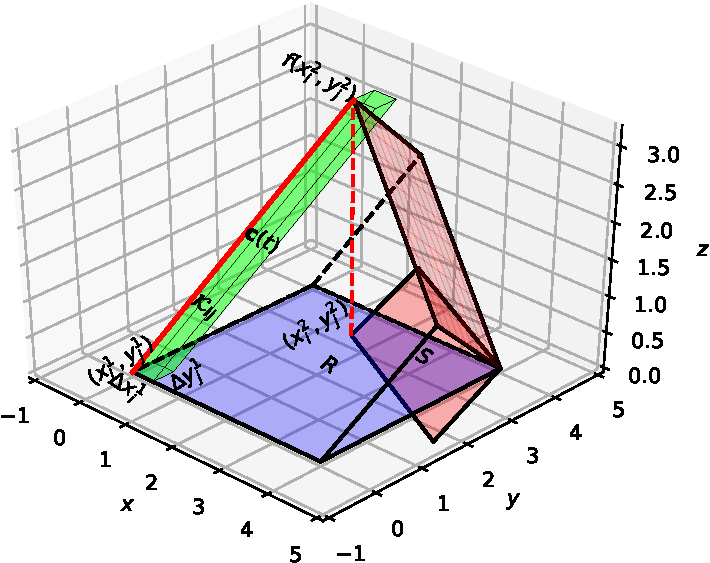
\includegraphics[width=0.75\textwidth]{prismatoid_solid.pdf}
\caption{xx}
\label{fig:prismatoid_solid}
\end{figure}

\begin{figure}[htb]
\centering
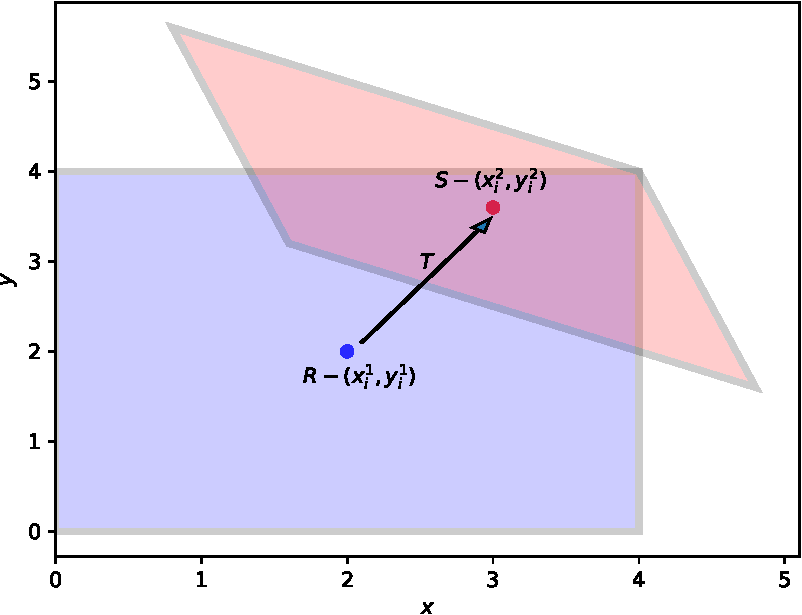
\includegraphics[width=0.75\textwidth]{prismatoid_regions.pdf}
\caption{xx}
\label{fig:prismatoid_regions}
\end{figure}

\noindent
In this paper, we will refer to the aforementioned limit as the double Cavalieri integral and we will denote this integral as follows:

\begin{equation}
\label{eq:cav_2d}
\iint \limits_{\mathcal{C}} f(x,y)~dA = \lim_{n,m \rightarrow \infty}  \sum_{i=0}^{n-1} \sum_{j=0}^{m-1} f(x_i^2,y_j^2) \Delta x_i^1 \Delta y_j^1,
\end{equation}
with $\mathcal{C} = \{\mathbf{c}(t),R\}$. As is the case for the single Cavalieri integral, Equation~\eqref{eq:cav_2d} is difficult to evaluate in its current form. Luckily, the double 
Cavalieri integral can be converted into an equivalent double Riemann integral using the transformation $T$:

\begin{eqnarray}
\iint\limits_{\!\mathcal{C}} f(x,y) dA &=& \lim_{n,m\rightarrow \infty} \sum_{j=1}^n\sum_{i=1}^n f(x_{ij}^2,y_{ij}^2) \Delta x_{ij}^1\Delta y_{ij}^1\\
&=&  \lim_{n,m\rightarrow \infty} \sum_{j=1}^n\sum_{i=1}^n f(h(x_{ij}^1,y_{ij}^1),s(x_{ij}^1,y_{ij}^1)) \Delta x_{ij}^1\Delta y_{ij}^1\\
&=& \int_a^b\int_c^d f(h(x,y),s(x,y))~dx~dy.
\end{eqnarray}

\noindent
The only thing that now remains is to find expressions for $h$ and $s$. Note that, for every coordinate pair $(x_i^1,y_i^1)\in R$ and $(x_i^2,y_i^2)\in S$ there exists a unique $t\in \mathbb{R}$ such that 
\begin{equation}
\label{eq:vector_2}
\left< x_i^2, y_i^2, f(x_i^2,y_i^2) \right > = \left < x_i^1, y_i^1, 0 \right > + \left <c_x(t),c_y(t),c_z(t)\right >  
\end{equation}
The above equation can be re-expressed as:
\begin{equation}
c_z(t) = f(x_i^1 + c_x(t),y_i^1 + c_y(t)). 
\end{equation}
We can now solve for $t$ in terms of $x_i^1$ and $y_i^1$. If we substitute this solution into Equation~\ref{eq:vector_2} we obtain:
\begin{equation}
x_i^2 = h(x_i^1,y_i^1) = x_i^1 + c_x\circ t(x_i^1,y_i^1) 
\end{equation}
and 
\begin{equation}
y_i^2 = s(x_i^1,y_i^1) = y_i^1 + c_y\circ t(x_i^1,y_i^1). 
\end{equation}

\section{Prismatoid}
Let $\mathcal{S}$ be the solid which is bounded by the planes $f(x,y)=-x-y+8$, $2x$, $2(x-4)$, $y$, $y-4$ and the $xy$-plane. Solid $\mathcal{S}$ is depicted 
in Figure~\ref{fig:prismatoid_solid}, Figure~\ref{fig:prismatoid} and Figure~\ref{fig:prismatoid_real}. Solid $\mathcal{S}$ is a prismatoid, since all of its 
vertices lie in two parallel planes. Furthermore, all of its lateral faces are trapezoids or triangles. Note that, the line of intersection between $2x$ and $y$ is $\mathbf{c}(t) = -\left<\frac{1}{2}t,t,t\right>$.
The line $\mathbf{c}(t)$ is depicted and labelled in Figure~\ref{fig:prismatoid_solid}.

As we alluded to in the previous section we can calculate $V_{\mathcal{S}}$ using the double Cavalieri integral:
\begin{equation}
\iint\limits_{\!\mathcal{C}} f(x,y) dA =  \int_a^b\int_c^d f(h(x,y),s(x,y))~dx~dy,
\end{equation}
with $\mathcal{C}=\{\mathbf{c}(t),R\}$. We can, however, only evaluate the above integral if the transformation $T$ is known (see Figure ). We can find $T$ using Equation

Let $\mathbf{c}(t) = -\left<\frac{1}{2}t,t,t\right>$ be the line of intersection between the planes $2x$ and $y$. Furthermore, note that the line 
$\mathbf{c}(t)$ passes through the origin. The line $\mathbf{c}(t)$ is depicted and labelled in Figure~\ref{fig:prismatoid_solid}. Let 
\begin{equation}
R = \{(x,y)\in\mathbb{R}^2|0 \geq x \geq 4, 0 \geq x \geq 4\} \nonumber
\end{equation}
and
\begin{equation}
S = \{(x,y)\in\mathbb{R}^2|-\sfrac{1}{3}y+\sfrac{8}{3}\leq x\leq -\sfrac{1}{3}y+\sfrac{16}{3}, \sfrac{1}{2} x + 4\leq y \leq \sfrac{1}{2} x + 6 \}. \nonumber
\end{equation}
The region $S$ and $R$ are depicted in Figure~\ref{fig:prismatoid_solid} and Figure~\ref{fig:prismatoid_regions}. Let us now subdivide $R$ into $n\times m$
subrectangles $R_{ij} = [x_{i},x_{i+1}] \times [y_{j},y_{j+1}]$ of equal width $\Delta x^1 = \Delta x_i^1 = x_{i+1}-x_i<<(b-a)$ and length $\Delta y^1= \Delta y_j^1 = y_{j+1}-y_j<<(d-c)$. 
Furthermore, let the transformation $T$ map the $xy$--coordinate $(x_i^1,y_i^1)\in R$ (the lower left vertice of $R_{ij}$) at which $\mathbf{c}(t) + \left <x_i^1,y_i^1,0 \right >$ intersects the 
$xy$-plane to the $xy$--coordinate $(x_i^2,y_j^2)\in S$ at which $\mathbf{c}(t) + \left <x_i^1,y_j^1,0 \right >$ intersects $f(x,y)$ (Figure~\ref{fig:prismatoid_solid} and Figure~\ref{fig:prismatoid_regions}). 
%The transformation $T$ is defined by the following equations:
%\begin{equation}
%x_i^2 = h(x_i^1,y_i^1)
%\end{equation}
%and
%\begin{equation}
%y_i^2 = s(x_i^1,y_i^1)
%\end{equation}

%Let $S_f = \{(x,y,z)\in\mathbb{R}^3|(x,y)\in S ~ \textrm{and} ~ z=f(x,y)\}$. Note that in $\mathbb{R}^3$, $R$ has the following vertices $\mathbf{v}_{R} = \{(x,y,z)\in\mathbb{R}^3|x\in\{a,b\},y\in\{c,d\}~\textrm{and}~z=0\}$,
%while $S_f$ has the following vertices $\mathbf{v}_{S_f} = \{(x,y,z)\in\mathbb{R}^3|x\in\{a,b\},y\in\{c,d\}~\textrm{and}~z=f(h(x,y),s(x,y))\}$. 

We can easily compute $V_{\mathcal{S}}$ using the 
volume equation of a prismatoid. The details of this computation is described in the caption of Figure~\ref{fig:prismatoid}. According to the prismatoid volume 
equation $V_{\mathcal{S}}=25.6$.\\















$R = \{(x,y)\in\mathbb{R}^2|0 \geq x \geq 4, 0 \geq x \geq 4\}$
and $S = \{(x,y)\in\mathbb{R}^2|-\sfrac{1}{3}y+\sfrac{8}{3}\geq x\leq -\sfrac{1}{3}y+\sfrac{16}{3} \}$.



The line $\mathbf{c}(t)$  is depicted and labelled in 


\begin{figure}[htb]
\centering
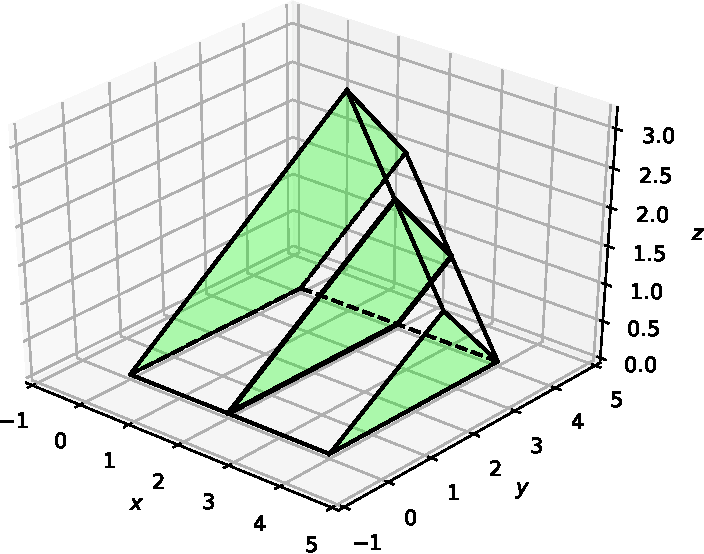
\includegraphics[width=0.75\textwidth]{prismatoid.pdf}
\caption{xx}
\label{fig:prismatoid}
\end{figure}

\begin{figure}[htb]
\centering
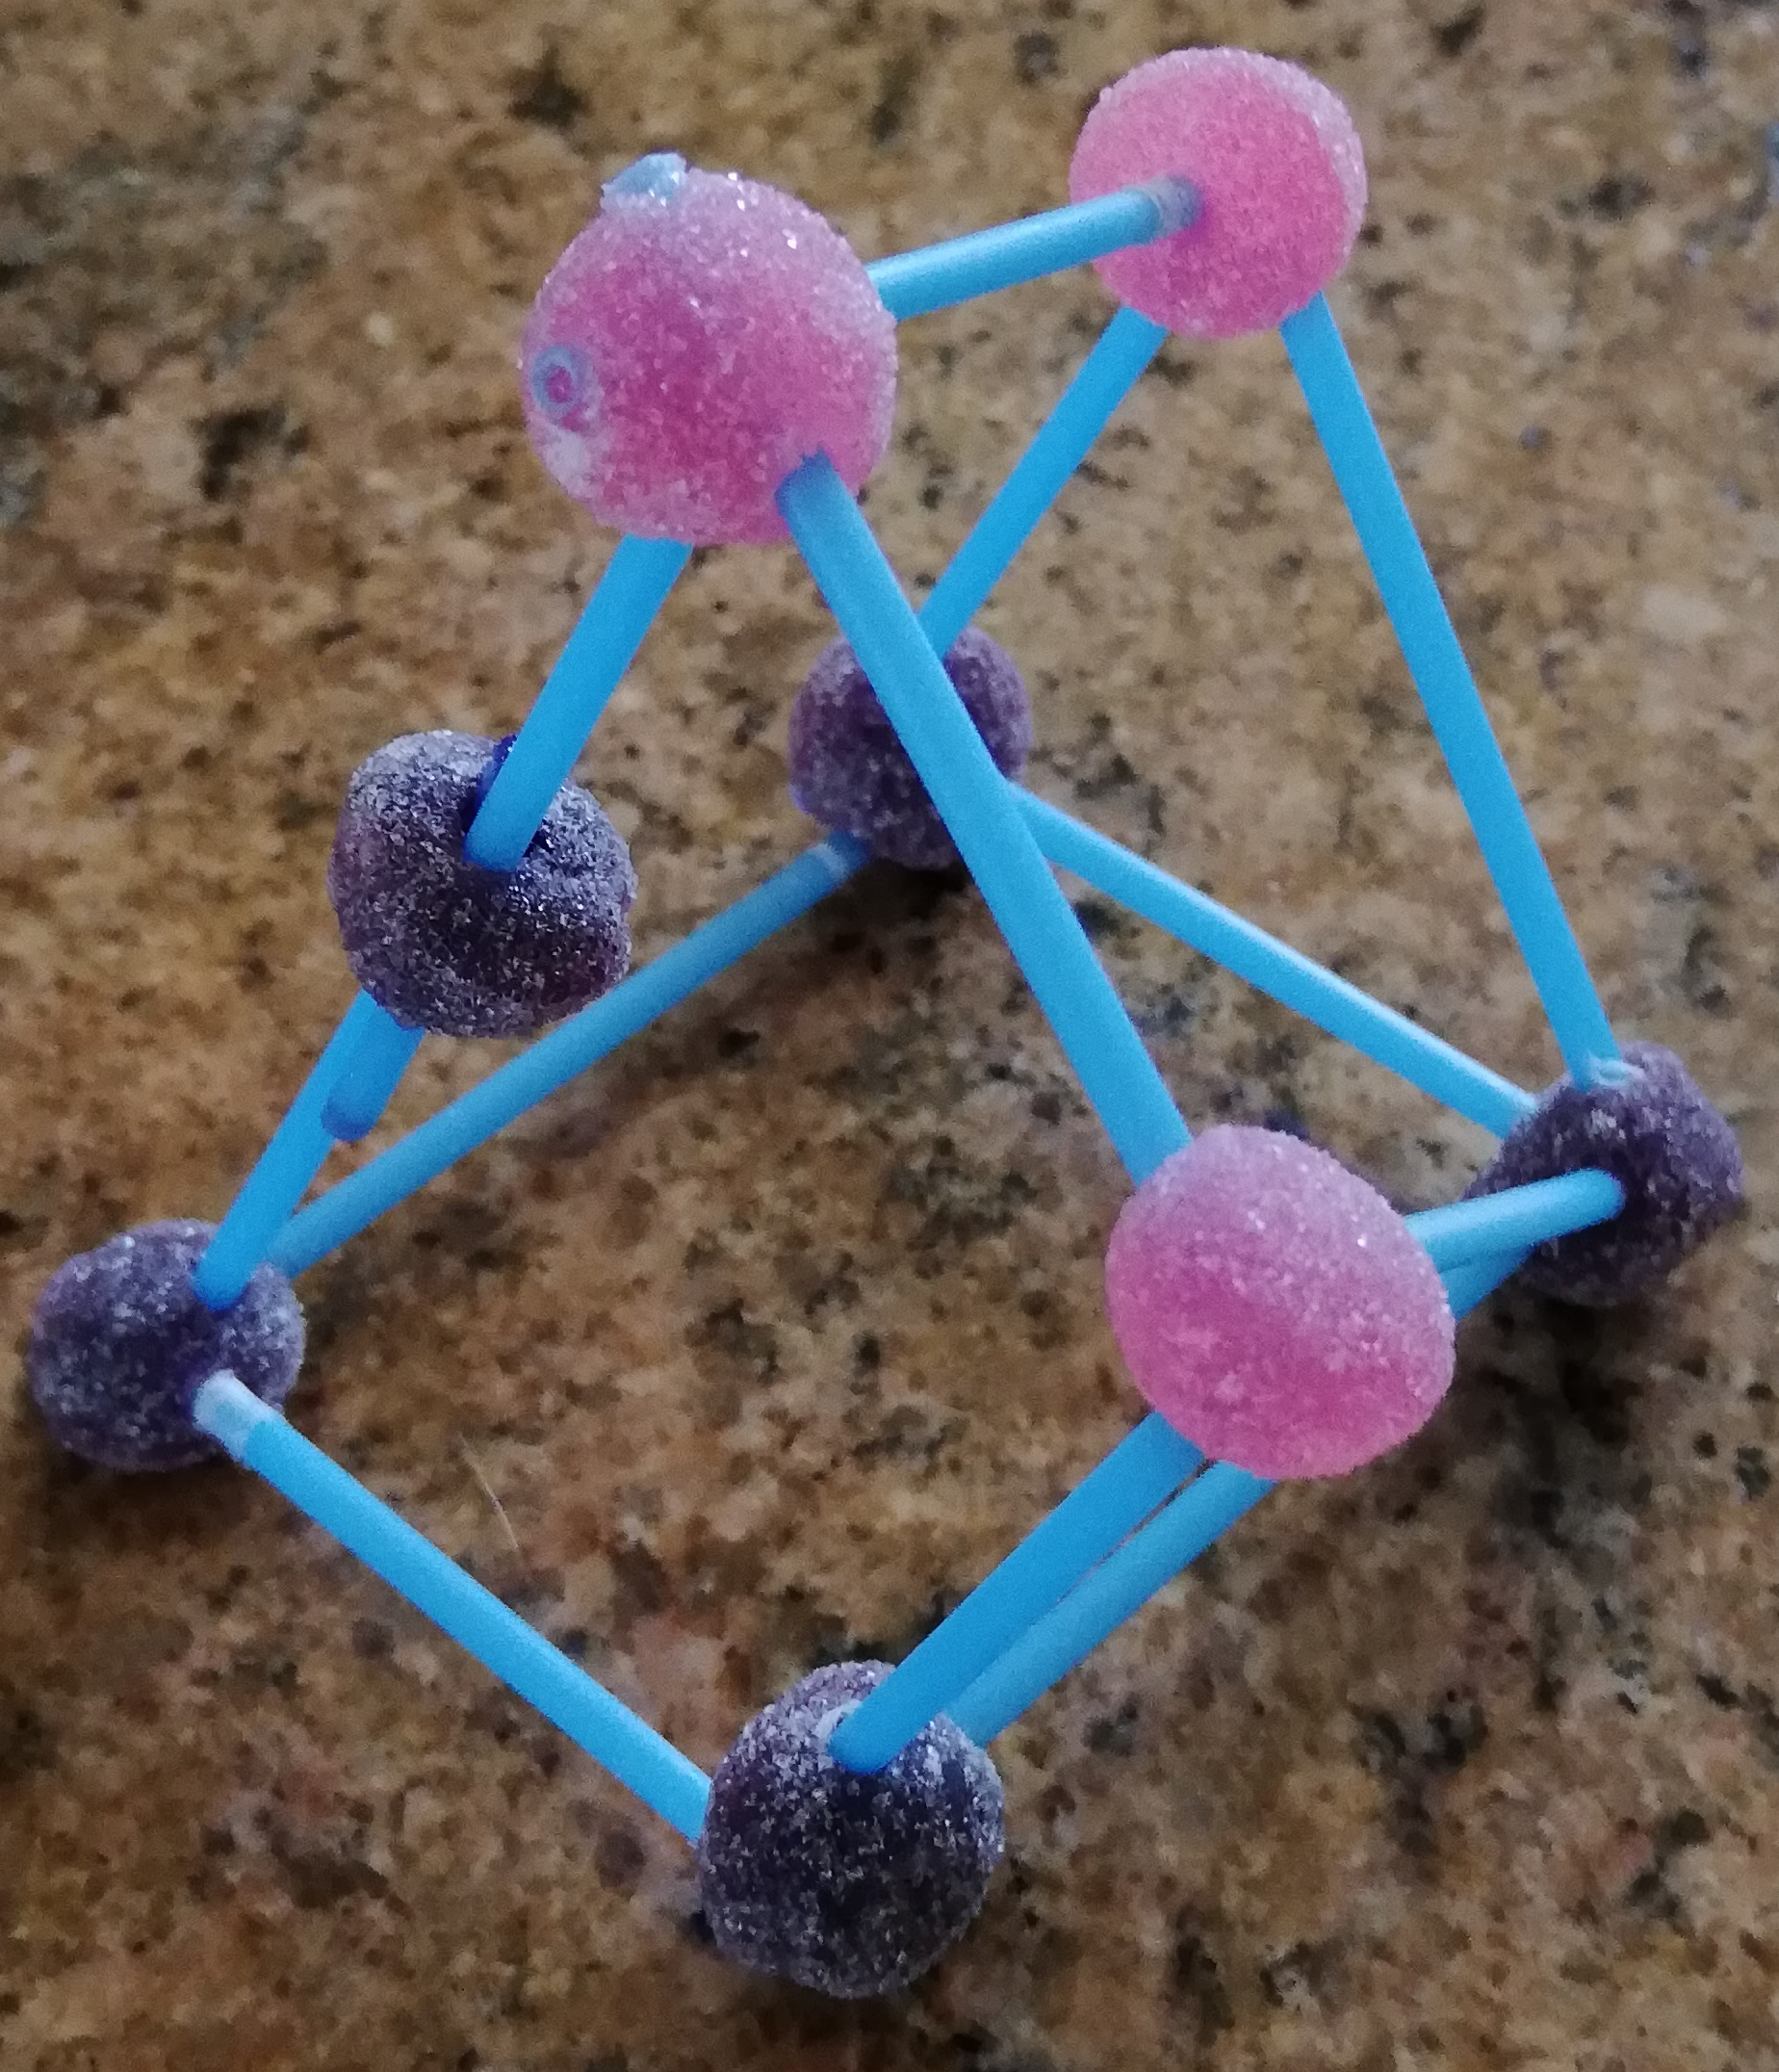
\includegraphics[width=0.5\textwidth]{prismatoid_real.jpg}
\caption{xx}
\label{fig:prismatoid_real}
\end{figure}

\begin{figure}[htb]
\centering
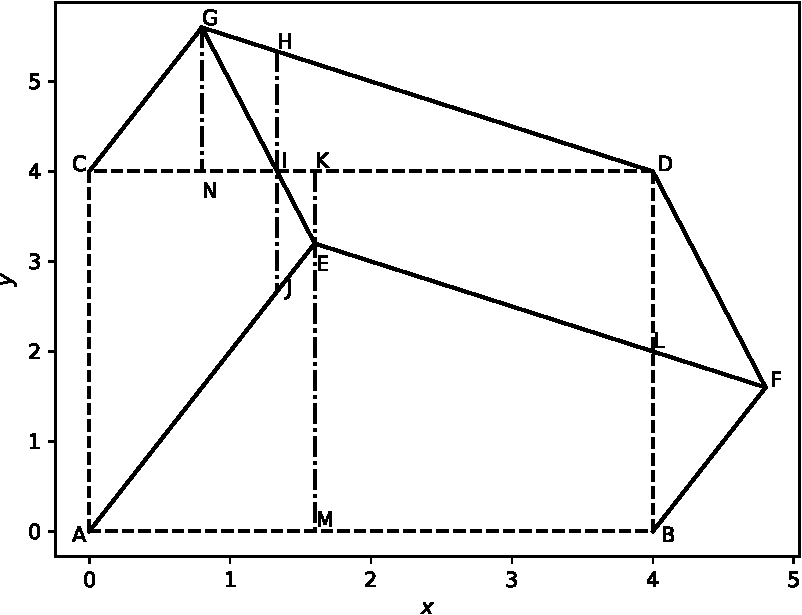
\includegraphics[width=0.75\textwidth]{prismatoid_xy.pdf}
\caption{xx}
\label{fig:prismatoid_xy}
\end{figure}

\begin{figure}[htb]
\centering
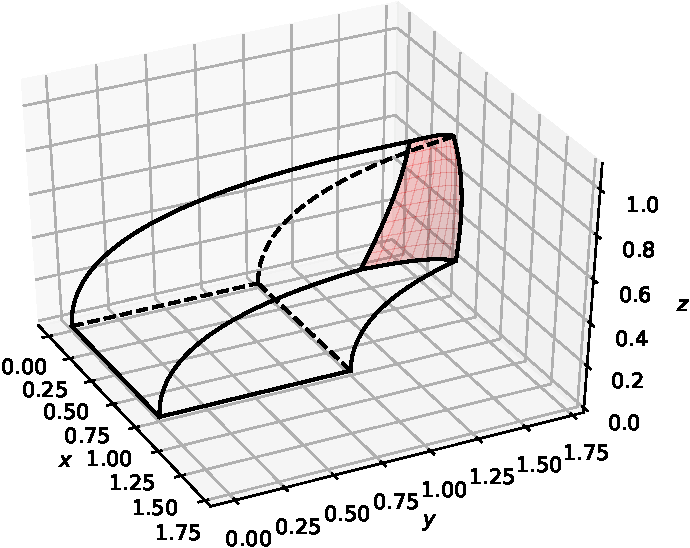
\includegraphics[width=0.75\textwidth]{sphere_solid.pdf}
\caption{xx}
\label{fig:sphere_solid}
\end{figure}

\begin{figure}[htb]
\centering
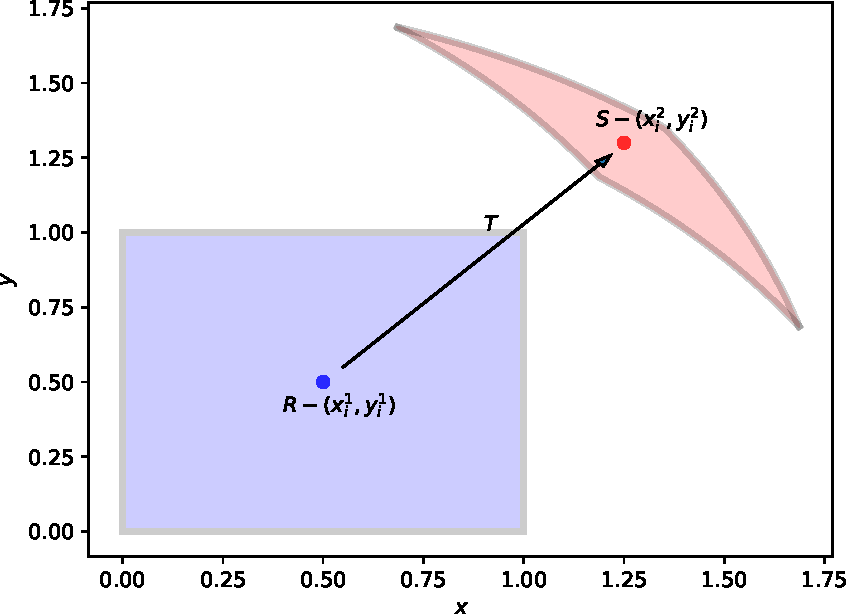
\includegraphics[width=0.75\textwidth]{sphere_regions.pdf}
\caption{xx}
\label{fig:sphere_regions}
\end{figure}

\begin{figure}[htb]
\centering
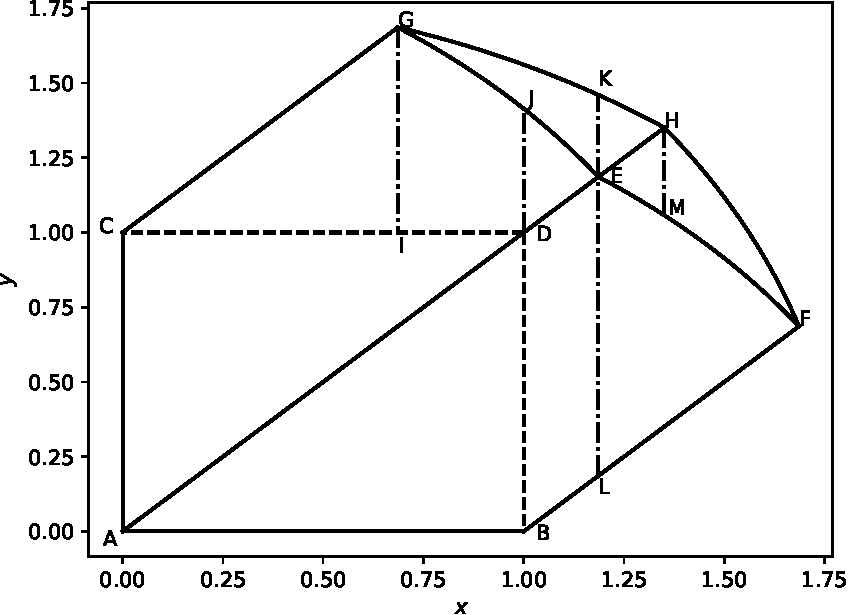
\includegraphics[width=0.75\textwidth]{sphere_xy.pdf}
\caption{xx}
\label{fig:sphere_solid}
\end{figure}




%in In turns out that $h$ can be constructed 
%as the reader progresses through the paper. As will become apparent later on in this paper defining your Cavalieri integral in terms of $\mathbf{c}(t)$ instead of 
%$a(y)$ makes it trivial to extend its defintion into $\mathbb{R}^3$.
%In Equation~\eqref{eq:new_def_cavalieri}, we denote the $\{\mathbf{c}(t),[a,b]\}$ via $\mathcal{C}$. Furthermore, $\mathbf{c}(t)$ denotes the vector equation of 
%$a(y)-a$.
%an alternative notation


% \noindent
% Intersestingly, the definition in Eq.~\eqref{??} can also be formulated via vector calculus notation. As will become apparent later on in the article extending the definition of the Cavalieri integral as it appears in ?? into $\mathbb{R}^3$ is problematic. However,
% if the definition in ?? is first re-expressed in vector calculus notation then it becomes trivial to extend it into $\mathbb{R}^3$.\\
% 
% \noindent
% We will now show that this is indeed the case. Note that, for every coordinate $(x_i^1,x_i^2) \in [a,b] \times [a',b']$ there exists a unique $t\in\mathbb{R}$ such that
% \begin{equation}
% \label{eq:pat_rel}
% \left <x_i^2,f(x_i^2) \right > = \left <x_i^1,0 \right> + \left<c_x(t),c_y(t) \right >.
% \end{equation}
% We can rewrite Equation~\eqref{eq:pat_rel} as
% \begin{equation}
% \label{eq:t_func}
% c_y(t) = f(x_i^1 + c_x(t)).
% \end{equation}
% We can now solve for $t$ in Equation~\eqref{eq:t_func} in terms of $x_i^1$. If we substitute the solution $t(x_i)$ into Equation~\ref{eq:pat_rel} we obtain
% \begin{equation}
% \label{eq:h_func}
% x_i^2 = x_i^1 + c_x\circ t(x_i^1).
% \end{equation}
% Note that Equation~\eqref{eq:h_func} is nothing more than the function $h$ expressed in terms of $t$, i.e. $x_i^2 = h(x_i^1) = x_i^1 + c_x\circ t(x_i^1)$.
% We can, therefore compute $h(x)$ from $\mathbf{c}(t)$ and as such we can can define the Cavalieri integral in terms of $\mathbf{c}(t)$ instead of $a(y)$. In light 
% of this observation we propose the following alternative notation to denote a Cavalieri integral 
% \begin{equation}
% \int  
% \end{equation}


% and as such $t(x_i^1)$ can be used to determine $h(x_i^1)$.
% i.e. $t$ is a function 
% It is therefore possible to define $t$ in terms of $x_i^1$.  
% \noindent
% Expressing \eqref{eq:caval1} in vector calculus notation
% \begin{equation}
% \int_{a(y)}^{b(y)}f(x)\, dx =\cint_a^b f(x)~dx, 
% \end{equation}
% with $\mathbf{c}(t) = <c_x(t),c_y(t)>$ denoting a vector equation that passes through the origin and is a translation of $a(y)$. We can express $a(y)$ as $\mathbf{c}(t) + <a,0>$.
% Note that partition $x_i^1$ and $x_i^2$ are related to each other via: 
% \begin{equation}
% \label{eq:pat_rel}
% <x_i^2,f(x_i^2)> = <x_i^1,0> + <c_x(t),c_y(t)> 
% \end{equation}
% It follows from Eq.~\eqref{eq:pat_rel} that 
% \begin{equation}
% c_y(t) = f(x_i^1 + c_x(t)). 
% \end{equation}
% We can therefore express $t$ as a function of $x_i^1$. We can now compute $h(x_i^1) = x_i^1 + t(x_i^1)$.








 






%One first divides a complex planar figure whose area is unknown into indivisible parallel chords. These cords are then translated 
%in such a way that the original planar figure is transformed into a planar figure whose area is easily computable. The volume of a complex solid can be computed 
%in a similar manner. 
%In this method areas of complex planar figures are computed by dividing such figures into indivisible parallel chords. One then 
%finds another planar figure whose area is known that consists of the exact same set of chords. The area of the complex planar figure is then 
 


\begin{abstract}
We presented a novel geometric interpretation of the Riemann-Liouville fractional integral. We found that a Riemann-Liouville integral can 
be thought of as the area obtained by summing together the area of an infinite number of non-rectangular infinitesimals whose shape is determined by the 
order of integration $\alpha$ and the integration limit $t$. We also showed that this geometric interpretation offers many pedagogical benefits as it is very similar
in nature to the geometric interpretation of the Riemann integral.   
\end{abstract}

\begin{thebibliography}{1}

\bibitem{ackermann12} Ackermann,~E.~R, Grobler,~T.~L., Kleynhans,~W., Olivier,~J.~C., Salmon,~B.~P, van Zyl,~A.~J. (2012). Cavalieri
Integration. \textit{Quaest. Math.} 35(3): 265–296.

\bibitem{adda97} Adda,~F.~B. (1997). Geometric interpretation of the fractional derivative. \textit{J. of Fract. Calc.}, 11: 21--52.

\bibitem{bartle76} Bartle,~R.~G. (1976). \textit{The Elements of Real Analysis.} New York: Wiley.

%Physical
\bibitem{cioc16} Cioc, R. (2016). Physical and geometrical interpretation of Gr\"{u}nwald-Letnikov differintegrals: Measurement of path and acceleration. \textit{Fract. Calc. Appl. Anal.} 19(1): 161--172.

\bibitem{davis59} Davis,~P.~J. (1959). Leonhard Euler's Integral: A Historical Profile of the Gamma Function. \textit{Amer. Math. Monthly}. 66(10): 849--869

\bibitem{euler1738} Euler,~L. (1738). De progressionibus transcendentibus seu quarum termini generales algebraice dari nequeunt. \textit{Commentarii academiae scientiarum Petropolitanae}. 36--57.

\bibitem{gomez14} Gomez-Aguilara,~J.~F., Razo-Hernandez,~R., Granados-Lieberman, D.~ A (2014). Physical interpretation of fractional
calculus in observable terms: analysis of the fractional time constant and the transitory response. \textit{Revista Mexicana de Fisica.} 60: 32--38

\bibitem{grobler19} Grobler,~T.~L. (2019). Visualization of the Riemann-Stieltjes integral. \textit{Coll. Math. J.} 50(3): 198--209.

\bibitem{laurent1884} Laurent,~H. (1884). Sur le calcul des d\'{e}riv\'{e}es \`{a} indices quelconques. \textit{Nouv Annales de Mathem\'{e}matiques.} 3(3):240--252. 

\bibitem{liouville1832} Liouville,~J. (1832). M\'{e}moire sur l\textquotesingle integration de l\textquotesingle \'{e}quation $(mx^2+nx+p)\frac{d^2y}{dx^2}+(qx+r)\frac{dy}{dx}+sy$ \`{a} l\textquotesingle aide des diff\'{e}rentielles \`{a} indices 
que\textquotesingle conques. \textit{Journal d l\textquotesingle Ecole Polytechnique.} 13(21): 163--186. 

\bibitem{machado03} Machado,~J.~T. (2003). A probabilistic interpretation of the fractional-order differentiation. \textit{Fract. Calc. Appl. Anal.} 6(1): 73--80.

\bibitem{machado14} Machado,~J.~T., Galhano,~A.~M., Trujillo,~J.~J. (2014). On development of fractional calculus during the last fifty years. \textit{Scientometrics}. 98(1): 577-582.

\bibitem{machado17} Machado,~J.~T., Kiryakova,~V. (2017). The chronicles of fractional calculus. \textit{Fract. Calc. Appl. Anal.} 20(2): 307--336.

\bibitem{munkhammar05} Munkhammar,~J. (2005). Fractional calculus and the Taylor-Riemann series. \textit{Rose-Hulman Undergrad. Math. J.}, 6(1): 6.

%physical
\bibitem{nigmatullin92} Nigmatullin,~R.~R (1992). A fractional integral and its physical interpretation. \textit{Theor. and Math. Phys.} 90(3): 242--251.

\bibitem{podlubny02} Podlubny,~I. (2002). Geometric and Physical Interpretation of Fractional Integration and Fractional Differentiation, \textit{Fract. Calc. Appl. Anal.} 5(4): 367--386.

\bibitem{riemann1876} Riemann,~B.~G.~F (1876). Gesammelte Werke.

\bibitem{ross77} Ross,~B. (1977). The development of fractional calculus 1695--1900. \textit{Hist. Math.} 4(1): 75--89.

\bibitem{ross06} Ross,~B. (Ed.). (2006). \textit{Fractional calculus and its applications: proceedings of the international conference held at the University of New Haven, June 1974}, Vol. 457, Springer.
 
\bibitem{rutman95} Rutman,~R.S. (1995). On physical interpretations of fractional integration and differentiation. \textit{Theor. and Math. Phys.} 105(3):1509--1519

 %Probability
\bibitem{stanislavsky04} Stanislavsky,~A.~A. (2004).  Probability interpretation of the integral of fractional order, \textit{Theor. and Math. Phys.} 138(3): 418--431.

%Geometric
\bibitem{tarasov16} Tarasov,~V.~E. (2016). Geometric interpretation of fractional-order derivative. \textit{Fract. Calc. Appl. Anal.} 19(5): 1200--1221.

%Economic
\bibitem{tarasova17} Tarasova,~V.~V., Tarasov,~V.~E. (2017). Economic Interpretation of Fractional Derivatives. \textit{Prog. in Fract. Diff. and Appl.} 3(1):1--7. 

\end{thebibliography}
\vfill\eject

\end{document}
